\section{Overview}

\begin{frame}\frametitle{General Ideas}
\begin{itemize}
\item Recall
 \begin{itemize}
 \item syntax = context-free grammar
 \item semantics = translation to another language
 \end{itemize}
\item Example: BOL translated to SQL, SFOL, Scala, English
\item Querying = use semantics to answer questions about syntax
\end{itemize}
\medskip

Note:
\begin{itemize}
\item Not the standard definition of querying
\item Design of a new Tetrapod-level notion of querying
 \glec{ongoing research}
\item Subsumes concepts of different names from the various aspects
\end{itemize}
\end{frame}

\begin{frame}\frametitle{Propositions}
syntax with propositions = \\
designated non-terminals for propositions
\medskip

Examples:
\begin{center}
\footnotesize
\begin{tabular}{l|l}
aspect & basic propositions\\
\hline
ontology language & assertions, concept equality/subsumption\\
programming language & equality for some types\\
database language & equality for base types \\
logic & equality for all types\\
natural language & sentences \\
\end{tabular}
\end{center}

Aspects vary critically in how propositions can be formed
\begin{itemize}
\item any program in computation
\item quantifiers in deductions \glec{undecidable}
\item $IN$ in databases
\end{itemize}
\end{frame}

\begin{frame}\frametitle{Propositions as Queries}
Propositions allow defining queries

\begin{center}
\footnotesize
\begin{tabular}{l|ll}
& Query & Result\\
\hline
deduction & proposition & yes/no \\
concretization & proposition with free variables & true ground instances \\
computation & term & value \\
narration & question & answer \\
\end{tabular}
\end{center}
\end{frame}

\begin{frame}\frametitle{Semantics of Propositions}
syntax with propositions = \\
designated non-terminals for propositions \\
\lec{needed to ask queries}
semantics with theorems = \\
designates some propositions as theorems or contradictions
\lec{needed to answer queries}

Note:
\begin{itemize}
\item A propositions may be neither theorem nor contradiction.
\item We say that language has negation if:\\ $F$ theorem iff $\neg F$ contradiction and vice versa.
\end{itemize}

We write $\vdash F$ if $F$ is theorem.
\end{frame}

\section{Deductive Queries}

\begin{frame}\frametitle{Definition}
We assume
\begin{itemize}
\item a semantics $\sem{-}$ from $l$ to $L$
\item $l$ has propositions
\item there is an operation $\truelift$ that maps translations of $l$-propositions to $L$-propositions
\item $L$ has semantics with propositions
\end{itemize}

We define
\begin{itemize}
\item a deductive query is an $l$-proposition $p$
\item the result is
 \begin{itemize}
 \item yes if $\truelift \sem{p}$ is a theorem of $L$
 \item no if $\truelift \sem{p}$ is a contradiction in $L$
 \end{itemize}
\end{itemize}
\end{frame}

\begin{frame}\frametitle{The $\truelift$ operator}
\begin{blockitems}{Problem with type-preserving translation $\sem{-}$}
\item must translate $F:\prop^l$ to $\sem{F}:\sem{\prop^l}$
\item but need not satisfy $\sem{\prop^l}=\prop^L$ \\
  \glec{$l$-propositions maybe not translated to $L$-propositions}
\item If not, $\vdash^L \sem{F}$ cannot be used to answer query $\vdash^l F$
\end{blockitems}

\begin{blockitems}{Solution: $L$-operator $\truelift: \sem{\prop^l}\to \prop^L$}
\item maps translations of $l$-propositions to $L$-propositions
\item then use $\vdash^L \truelift \sem{F}$ to answer $\vdash^l F$
\end{blockitems}

\begin{blockitems}{Example: standard semantics of SFOL in set theory}
\item SFOL-propositions: formulas; set theory propositions: truth values
\item semantics of formula is function from models to truth values
\item $\truelift$ takes $\sem{F}$ and returns $1$ iff $\sem{F}(M)=1$ for all models $M$
 \glec{standard notation for $\sem{F}(M)=1$: $\sem{F}^M=1$ or $M\models F$}
\end{blockitems}
\end{frame}
  
\begin{frame}{Breakout question}
What can go wrong?
\end{frame}

\begin{frame}\frametitle{Problem: Inconsistency}
In general, (in)consistency of semantics
\begin{itemize}
\item Some propositions may be both a theorem and a contradiction.
\item In that case, queries do not have a result.
\end{itemize}

In practice, however:
\begin{itemize}
\item If this holds for some propositions, it typically holds for all of them.
\item In that, we call $L$ inconsistent.
\item We usually assume $L$ to be consistent.
\end{itemize}
\end{frame}


\begin{frame}\frametitle{Problem: Incompleteness}
In general, (in)completeness of semantics
\begin{itemize}
\item We cannot in general assume that every proposition in $L$ is either a theorem or a contradiction.
\item In fact, most propositions are neither.
\item So, queries do not necessarily have a result.
\item We speak of incompleteness. \glec{Note: not the same as the usual (in)completeness of logic}
\end{itemize}

In practice, however:
\begin{itemize}
\item It may be that $L$ is complete for all propositions in the image of $\truelift\sem{-}$.
\item This is the case if $l$ is simple enough \glec{typical for ontology languages}
\end{itemize}
\end{frame}

\begin{frame}\frametitle{Problem: Undecidability}
In general, (un)decidability of semantics:
\begin{itemize}
\item We cannot in general assume that it is decidable whether a proposition in $L$ is a theorem or a contradiction.
\item In fact, it usually isn't.
\item So, we cannot necessarily compute the result of a query.
\item However: If we have completeness, decidability is likely.
 \glec{run provers for $F$ and $\neg F$ in parallel}
\end{itemize}

In practice, however:
\begin{itemize}
\item It may be that $L$ is decidable for all propositions in the image of $\truelift\sem{-}$.
\item This is the case if $l$ is simple enough \glec{typical for ontology languages}
\end{itemize}
\end{frame}

\begin{frame}\frametitle{Problem: Inefficiency}
In general, (in)efficiency of semantics:
\begin{itemize}
\item Answering deductive queries is very slow.
\item Even if we are complete and decidable.
\end{itemize}

In practice, however:
\begin{itemize}
\item Decision procedures for the image of $\truelift\sem{-}$ may be quite efficient.
\item Dedicated implementations for specific fragments.
\item This is the case if $l$ is simple enough \glec{typical for ontology languages}
\end{itemize}
\end{frame}

\section{Contexts and Free Variables}

\begin{frame}\frametitle{Concepts}
Recall the analogy between grammars and typing:

\begin{center}
\begin{tabular}{l|l}
grammars & typing \\
\hline
non-terminal & type \\
production & constructor \\
non-terminal on left of production & return type of constructor \\
non-terminals on right of production & arguments types of constructor \\
terminals on right of production & notation of constructor\\
words derived from non-terminal $N$ & expressions of type $N$
\end{tabular}
\end{center}

We will now add contexts and substitutions.
\end{frame}

\begin{frame}\frametitle{Contexts}
Independent of whether $l$ already has contexts/variables, we can define:
\begin{itemize}
 \item A \emph{context} $\Gamma$ is of the form $x_1:N_1,\ldots,x_n:N_n$ where the
  \begin{itemize}
   \item $x_i$ are names
   \item $N_i$ are non-terminals
  \end{itemize}
  We write this as $\vdash_l \Gamma$.
 \item A \emph{substitution} for $\Gamma$ is of the form $x_1:=w_1,\ldots,x_n:=w_n$ where the
  \begin{itemize}
   \item $x_i$ are as in $\Gamma$
   \item $w_i$ derived from the corresponding $N_i$
  \end{itemize}
  We write this as $\vdash_l \gamma:\Gamma$.
 \item An \emph{expression in context} $\Gamma$ of type $N$ is a word $w$ derived from $N$ using additionally the productions $N_i::= x_i$.\\
 We write this as $\Gamma\vdash_l w:N$.
 \item Given $\Gamma\vdash w:N$ and $\vdash \gamma:\Gamma$ as above, the \emph{substitution of} $\gamma$ in $w$ is obtained by replacing every $x_i$ in $w$ with $w_i$.
 We write this as $w[\gamma]$.
\end{itemize}
\end{frame}


\begin{frame}\frametitle{Contexts under Compositional Translation}
Consider a compositional semantics $\sem{-}$ from $l$ to $L$ between context-free languages.

\begin{itemize}
 \item Every $\vdash_l w:N$ is translated to some $\vdash_L \sem{w}:N'$ for some $N'$.
 \item Compositionality ensures that $N'$ is the same for all $w$ derived from $N$.
 \item We write $\sem{N}$ for that $N'$.
 \item Then we have 
  \[\vdash_l w:N \tb\mimplies\tb \vdash_L \sem{w}:\sem{N}\]
\end{itemize}

Now we translate contexts, substitutions, and variables as well:
\[\sem{x_1:N_1,\ldots,x_n:N_n}:=x_1:\sem{N_1},\ldots,x_n:\sem{N_n}\]
\[\sem{x_1:=w_1,\ldots,x_n:=w_n}:=x_1:=\sem{w_1},\ldots,x_n:=\sem{w_n}\]
\[\sem{x}:=x\]

Then we have
  \[\Gamma\vdash_l w:N \tb\mimplies\tb \sem{\Gamma}\vdash_L \sem{w}:\sem{N}\]
\end{frame}

\begin{frame}\frametitle{Substitution under Compositional Translation}
From previous slide:
\[\sem{x_1:N_1,\ldots,x_n:N_n}:=x_1:\sem{N_1},\ldots,x_n:\sem{N_n}\]
\[\sem{x_1:=w_1,\ldots,x_n:=w_n}:=x_1:=\sem{w_1},\ldots,x_n:=\sem{w_n}\]
\[\sem{x}:=x\]
\[\Gamma\vdash_l w:N \tb\mimplies\tb \sem{\Gamma}\vdash_L \sem{w}:\sem{N}\]

We can now restate the substitution theorem as follows:
  \[\sem{E[\gamma]}=\sem{E}[\sem{\gamma}]\]
\end{frame}

\section{Concretized Queries}

\begin{frame}\frametitle{Definition}
We assume
\begin{itemize}
\item as for deductive queries
\item semantics must be compositional
\end{itemize}

We define
\begin{itemize}
\item a concretized query is an $l$-proposition $p$ in context $\Gamma$
\item a \emph{single} result is a
 \begin{itemize}
 \item a substitution $\vdash_l \gamma:\Gamma$
 \item such that $\vdash_L \truelift \sem{p[\gamma]}$
 \end{itemize}
\item the \emph{result set} is the set of all results
\end{itemize}
\end{frame}

\begin{frame}\frametitle{Example}
\begin{enumerate}
\item BOL ontology:
\[\mathll{concept\, male,\; concept\, person,\;axiom\, male \sqsubseteq person, \\
  individual\, FlorianRabe,\;assertion\, FlorianRabe\, isa\, male}\]
\item Query $x:individual\vdash_{BOL}x \text{ isa } person$
\item Translation to SFOL: $x:\iota\vdash_{SFOL} person(x)$
\item SFOL calculus yields theorem $\vdash_{SFOL}person(FlorianRabe)$
\item Query result $\sem{\gamma}= x:= FlorianRabe$
\item Back-translating the result to BOL: $\gamma= x:= FlorianRabe$
 \glec{back translation is deceptively simple:}
 \glec{translates SFOL-constant to BOL-individual of same name}
\end{enumerate}
\end{frame}

\begin{frame}{Breakout question}
What can go wrong?
\end{frame}

\begin{frame}\frametitle{Problem: Open World}
In general, semantics uses open world:
\begin{itemize}
\item open world: result contains \emph{all known} results
 \lec{same query might yield more results later}
\item closed world: result set contains \emph{all} results
\end{itemize}
 \glec{always relative to concrete database for $L$}

In practice, however,
\begin{itemize}
\item system explicitly assumes closed world
 \glec{typical for databases}
\item users aware of open world and able to process results correctly
\end{itemize}
\end{frame}

\begin{frame}\frametitle{Problem: Infinity of Results}
In general, there may be infinitely many results:
\begin{itemize}
\item e.g., query for all $x$ such that $\vdash x$,
\end{itemize}

In practice, however,
\begin{itemize}
\item systems pull results from finite database \lec{e.g., SQL, SPARQL}
\item systems enumerate results, require user to explicitly ask for more \lec{e.g., Prolog}
\end{itemize}
\end{frame}

\begin{frame}\frametitle{Problem: Back-Translation of Results}
In general, $\sem{-}$ may be non-trivial to invert
\begin{itemize}
\item easy to obtain $\sem{p}$ in context $\sem{\Gamma}$
  \glec{just apply semantics}
\item possible to find substitutions
\[\vdash_L \delta:\sem{\Gamma} \tb\mwhere\tb \sem{\Gamma}\vdash_L \truelift \sem{p}[\delta]\]
  \glec{easiest case: just look them up in database}
\item but how to translate $\delta$ to $l$-substitutions $\gamma$ with
 \[\vdash_l \gamma:\Gamma \tb\mwhere\tb \sem{\Gamma}\vdash_L \truelift \sem{p[\gamma]}\]
 substitution theorem: pick such that $\sem{\gamma}=\delta$
  \glec{the more $\sem{-}$ does, the harder to invert}
\end{itemize}

In practice, however:
\begin{itemize}
\item often only interested in concrete substitutions
\item translation of concrete data usually identity
\end{itemize}
But: practice restricted to what works even if more is needed
\end{frame}


\section{Computational Queries}

\begin{frame}\frametitle{Definition}
We assume
\begin{itemize}
\item the same as for deductive queries
\item semantics has equality/equivalence $\doteq$
\end{itemize}

We define
\begin{itemize}
\item a computational query is an $l$-expression $e$
\item the result is an $l$-expression $e'$ so that $\vdash_L\sem{e}\doteq\sem{e'}$
\end{itemize}
\lec{intuition: $e'$ is the result of evaluating $e$}

If semantics is compositional, $e$ may contain free variables
\lec{evaluate to themselves}
\end{frame}

\begin{frame}\frametitle{Problem: Back-Translation of Results}
In general, $\sem{-}$ may be non-trivial to invert
\begin{itemize}
\item easy to obtain $E:=\sem{e}$
\item possible to find $E'$ with $\vdash_L E'\doteq E$ by working in the semantics
\item non-obvious how to obtain $e'$ such that $\sem{e'}=E'$
\end{itemize}

In practice, however:
\begin{itemize}
\item evaluation meant to simplify, i.e., only useful if $E'$ very simple
\item simple $E'$ usually in the image of $\sem{-}$
\item typical case: $E'$ is concrete data and $e'=E'$ \lec{called a value}
\end{itemize}
\end{frame}

\begin{frame}\frametitle{Problem: Non-Termination}
In general, computation of $E'$ from $E$ might not terminate
\begin{itemize}
 \item while-loops
 \item recursion
 \item $(\lambda x. x\,x)\,(\lambda x. x\,x)$ with $\beta$-rule
 \item simplification rule $x\cdot y \rewrites y\cdot x$ \glec{similar: distributivity, associativity}
\end{itemize}

In practice, however:
\begin{itemize}
\item image of $\sem{-}$ part of terminating fragment
\end{itemize}
But: if $l$ is Turing-complete or undecidable, general termination not possible
\end{frame}

\begin{frame}\frametitle{Problem: Lack of Confluence}
In general, there may be multiple $E'$ that are simpler than $E$
\begin{itemize}
 \item there may be multiple rules that apply to $E$
 \item e.g., $f(g(x))$
  \begin{itemize}
  \item call-by-value: first simplify $g(x)\rewrites y$, then $f(y)\rewrites z$
  \item call-by-name: first plug $g(x)$ into definition of $f$, then simplify
  \end{itemize}
\item Normal vs. canonical form
 \begin{itemize}
 \item normal: $\vdash_L E\doteq E'$
 \item canonical: normal and $\vdash_L E_1\doteq E_2$ iff $E_1'=E_2'$
  \glec{equivalent expressions have identical evaluation}
  \glec{allows deciding equality}
 \end{itemize}
\end{itemize}

In practice, however:
\begin{itemize}
\item image of $\sem{-}$ part of confluent fragment
\item typical: evaluation to a value is canonical form
 \glec{works for BDL-types but not for, e.g., function types}
\end{itemize}
\end{frame}

\section{Narrative Queries}

\begin{frame}\frametitle{Definition}
We assume
\begin{itemize}
\item semantics into natural language
\end{itemize}

We define
\begin{itemize}
\item a narrative query is an $L$-question about some $l$-expressions
\item the result is the answer to the question
\end{itemize}
\end{frame}

\begin{frame}\frametitle{Problem: Unimplementable}
very expressive = very difficult to implement
\begin{itemize}
\item Natural language understanding
 \begin{itemize}
 \item no implementable syntax of natural language
  \glec{needs restriction to controlled natural language}
 \item specifying semantics hard even when controlled
 \end{itemize}
\item Knowledge base for question answering needed
 \begin{itemize}
 \item very large \glec{must include all common sense}
 \item might be inconsistent \glec{common sense often is}
 \item finding answers still very hard
 \end{itemize}
\end{itemize}
 
In practice, however:
\begin{itemize}
 \item accept unreliability \glec{attach probability measures to answers}
 \item implement special cases \glec{e.g., lookup in databases like Wikidata}
 \item search knowledge base for related statements \glec{Google, Watson}
\end{itemize}
\end{frame}


\section{Syntactic Querying}

\begin{frame}\frametitle{Search}
\begin{itemize}
\item ``search'' not systematically separated from ``querying''
\item often interchangeable
\item querying tends to imply formal languages for queries with well-specified semantics
 \lec{e.g., SQL}
\item search tends to imply less targeted process
 \lec{e.g., Google}
\end{itemize}
\lec{we will not distinguish between the two}
\end{frame}

\begin{frame}\frametitle{Syntactic vs. Semantic Querying}
\begin{blockitems}{Semantic querying}
\item Query results specified by vocabulary $V$ but (usually) not contained in it
\item Query answered using semantics of language
\item Challenge: apply semantics to find results
 \begin{itemize}
 \item deductive query $\vdash f:\prop$ requires theorem prover 
 \item computation query $\vdash e:E$ requires evaluator
 \item concrete query $\Gamma\vdash f:\prop$ requires enumerating all substitutions, running theorem prover/evaluator on all of them
 \end{itemize}
\end{blockitems}
\lec{what we've looked at so far}

\begin{blockitems}{Syntactic querying}
\item Query is an expression $e$
\item Result is set of occurrences of $e$ in $V$
\item Independent of semantics
\item Much easier to realize
\end{blockitems}
\end{frame}

\begin{frame}\frametitle{Challenges for Syntactic Search}
Easier to realize $\to$ scale until new challenges arise
\begin{itemize}
\item large vocabularies
 \begin{itemize}
 \item narrative: all text documents in a domain \glec{e.g., all websites, all math papers}
 \item deductive: large repositories of formalization in proof assistants
  \glec{$10^5$ theorems}
 \item computational: package managers for all programming languages
 \item concrete: all databases in a domain \glec{TBs routine}
 \end{itemize}
\item incremental indexing: reindex only new/changed parts
\item incremental search to handle large result sets \glec{pagination}
\item sophisticated techniques for
 \begin{itemize}
 \item indexing: to allow for fast retrieval
 \item similarity: to select likely results
 \item quality: to rank selected results
\end{itemize}
\item integration of some semantic parts
\end{itemize}
\end{frame}

\begin{frame}\frametitle{Overview}
\begin{itemize}
\item Deduction 
 \begin{itemize}
 \item semantic: theorem proving called search
 \item syntactic: text search
 \end{itemize}
\item Concretization
 \begin{itemize}
 \item semantic: complex query languages (nestable queries)
  \glec{SQL, SPARQL}
 \item syntactic: search by identifier (linked data)
 \end{itemize}
\item Computation
 \begin{itemize}
 \item semantic: interpreters called execution
 \item mixed: IDEs search for occurrences, dependencies
 \item syntactic: search in IDE, package manager
\end{itemize}
\item Narration:
 \begin{itemize}
 \item semantic: very difficult
 \item syntactic: bag of words search
 \end{itemize}
\end{itemize}
\end{frame}


\begin{frame}\frametitle{Abstract Definition: Document}
\textbf{Document} =
\begin{itemize}
\item file or similar resource that contains vocabularies
\item often with comments, metadata
\item different names per aspect
\begin{itemize}
\item deduction: formalization, theory, article
\item computation: source files
\item concretization: database, ontology ABox
\item narrative: document, web site
\end{itemize}
\end{itemize}

\textbf{Library} =
\begin{itemize}
\item collection of documents
\item usually structured into folders, files or similar
\item often grouped by user access \glec{e.g., git repository}
\item vocabularies interrelated within and across libraries
\end{itemize}
\end{frame}

\begin{frame}\frametitle{Abstract Definition: Document Fragment}
\textbf{Fragment} = subdivision of documents into nested semantic units

Examples
\begin{itemize}
\item deductive: theory, section, theorem, definition, proof step, etc.
\item computational: class, function, command, etc.
\item concrete: table, row, cell
\item narrative: section, paragraph, etc.
\end{itemize}

Assign unique \textbf{fragment URI}, e.g., LIB/DOC?FRAG where
\begin{itemize}
\item LIB: base URI of library \lec{e.g., repository URL}
\item DOC: path to document within library \lec{e.g., folder structure, file name}
\item FRAG: id of fragment within document \lec{e.g., class name/method name}
\end{itemize}
\end{frame}

\begin{frame}\frametitle{Abstract Definition: Index(er)}
\textbf{Indexer} consists of
\begin{itemize}
\item data structure $O$ for indexable objects
 \lec{specific to aspect, index design}
 \glec{e.g., words, syntax trees}
\item function that maps library to index \glec{the indexing}
\end{itemize}

\textbf{Index entry} consists of
\begin{itemize}
\item object that occurred in the library
\item URI of the containing fragment
\item information on where in the fragment it was found
\end{itemize}

\textbf{Index} = set of index entries
\end{frame}

\begin{frame}\frametitle{Abstract Definition: Query and Result}
Given
\begin{itemize}
\item indexer $I$ with data structure $O$
\item set of libraries
\item union of their indexes  \lec{computed once, queried often}
\end{itemize}

\textbf{Query} = object $\Gamma \vdash^I q:O$

\textbf{Result} consists of
\begin{itemize}
\item index entry with object $o$
\item substitution for $\Gamma$ such that $q$ matches $o$
 \lec{definition of ``match'' index-specific, e.g., $q[\gamma]=o$}
\end{itemize}

\textbf{Result set} = set of all results in the index
\end{frame}

\begin{frame}\frametitle{Bag of Words Search}
Definition:
\begin{itemize}
\item Index data structure = sequences of words (n-grams) up to a certain length
\item Query = bag of words
 \glec{bag = multiset}
\item Match: (most) words in query occur in same n-gram or n-grams near each other
\end{itemize}

Example implementations
 \begin{itemize}
 \item internet search engines for websites
 \item Elasticsearch: open source engine for custom vocabularies
 \end{itemize}

Mostly used for narrative documents
\begin{itemize}
 \item can treat concrete values as words \glec{e.g., numbers}
 \item could treat other expressions as words \glec{works badly}
\end{itemize}

\end{frame}

\begin{frame}\frametitle{Symbolic Search}
Definition:
\begin{itemize}
\item Index data structure = syntax tree (of any grammar) of expressions $o$ with free/bound variables
\item Query = expression $q$ with free (meta-)variables
\item Match: $q[\gamma]=_\alpha o$, i.e., up to variable renaming
\end{itemize}

Example implementation
 \begin{itemize}
 \item MathWebSearch \lec{see separate slides on MathWebSearch in the repository}
 \end{itemize}

Mostly used for formal documents
\begin{itemize}
 \item deductive
 \item computational
\end{itemize}
\end{frame}

\begin{frame}\frametitle{Knowledge Graph Search}
Definition:
\begin{itemize}
\item Index data structure = assertion forming node/edge in a knowledge graph
\item Index = big knowledge graph $G$
\item Query = knowledge graph $g$ with free variables
\item Match: $g[\gamma]$ is part of $G$
\end{itemize}

Example implementations
 \begin{itemize}
 \item SPARQL engines without consequence closure \glec{i.e., the most common case in practice}
 \item graph databases
 \end{itemize}

Mainly used for ABoxes of untyped ontologies
\end{frame}

\begin{frame}\frametitle{Value Search}
Definition:
\begin{itemize}
\item Index data structure = BDL values $v$
\item Query = BDL expression $q$ with free variables
\item Match: $q[\gamma]=v$
\end{itemize}

Example implementations
 \begin{itemize}
 \item no systematic implementation yet
 \item special cases part of most database systems
 \end{itemize}

Could be used for values occurring in any document
\begin{itemize}
 \item all aspects
 \item may need to decode/encode before putting in index
\end{itemize}
\end{frame}

\begin{frame}\frametitle{Cross-Aspect Occurrences}
Observation
\begin{itemize}
\item libraries are written in one primary aspect
\item indexer focuses on one aspect and kind of object
\item but documents may contain indexable objects of any index
\end{itemize}
\end{frame}

\begin{frame}\frametitle{Cross-Aspect Occurrences: Examples}
\begin{itemize}
\item Any library can contain
\begin{itemize}
 \item metadata on fragments
  \begin{itemize}
  \item relation assertions induce knowledge graph structure between fragments
  \item property assertions contain values narrative, symbolic objects, or values
 \end{itemize}
 \item cross-references to fragments of any other library
 \item narrative comments
\end{itemize}
\item Narrative text may contain symbolic expressions \glec{STEM documents}
\item Database table may have columns containing
 \begin{itemize}
 \item text
 \item encoded BDL values
 \item symbolic expression (often as strings)
 \end{itemize}
\item Symbolic fragments may contain database references
 \glec{e.g., when using database for persistent memoization}
\end{itemize}
\end{frame}

\begin{frame}\frametitle{A New Indexing Design}
recent paper \url{https://kwarc.info/people/frabe/Research/BKR_mdql_20.pdf} \glec{with K. Bercic}

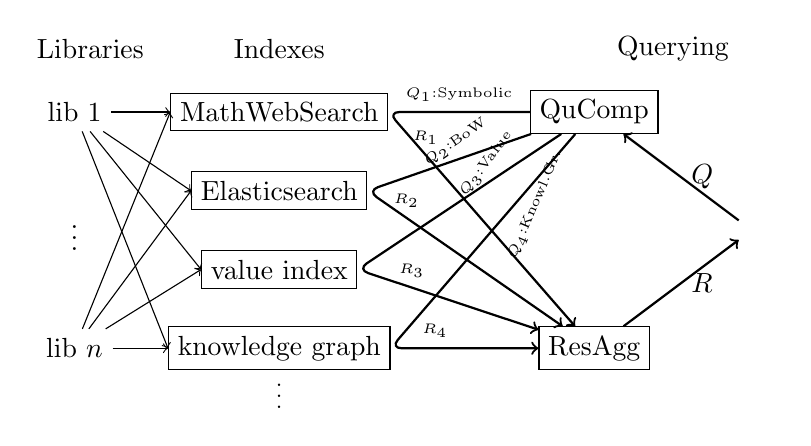
\begin{tikzpicture}[xscale=2]
  \node at (.8,2.8) {Libraries};
  \node (l1) at (0.7,2) {lib 1};
  \node at (.7,.5) {\vdots};
  \node (ln) at (0.7,-1) {lib $n$};
  \node at (2,2.8) {Indexes};
  \node[draw] (si) at (2,2) {MathWebSearch};
  \node[draw] (ni) at (2,1) {Elasticsearch};
  \node[draw] (ci) at (2,0) {value index};
  \node[draw] (oi) at (2,-1) {knowledge graph};
  \node (d) at (2,-1.5]) {\footnotesize\vdots};
  \draw[->] (l1) -- (si);
  \draw[->] (l1) -- (ni.west);
  \draw[->] (l1) -- (oi.west);
  \draw[->] (l1) -- (ci.west);
  \draw[->] (ln) -- (si.west);
  \draw[->] (ln) -- (ni.west);
  \draw[->] (ln) -- (ci.west);
  \draw[->] (ln) -- (oi.west);
  \node at (4.5,2.8) {Querying};
  \node[draw] (qc) at (4,2) {QuComp};
  \node[draw] (qa) at (4,-1) {ResAgg};

  \draw[->,rounded corners,thick] (qc) -- node[above] {\tiny $Q_1$:Symbolic}
                                             (si.east) -- node[pos=.2,above] {\tiny $R_1$} (qa);
  \draw[->,rounded corners,thick] (qc) -- node[pos=.4,above,sloped] {\tiny $Q_2$:BoW}
                                             (ni.east) -- node[pos=.2,above] {\tiny $R_2$} (qa); 
  \draw[->,rounded corners,thick] (qc) -- node[pos=.3,above,sloped] {\tiny $Q_3$:Value}
                                              (ci.east) -- node[pos=.3,above] {\tiny $R_3$} (qa); 
  \draw[->,rounded corners,thick] (qc) -- node[pos=.3,below,sloped] {\tiny $Q_4$:Knowl.Gr.}
                                              (oi.east) -- node[pos=.3,above] {\tiny$R_4$}(qa);

  \node[minimum width=.8cm] (u) at (5,.5) {};

  \draw[->,thick] (u) -- node[right] {$Q$} (qc);
  \draw[->,thick] (qa) -- node[right] {$R$} (u);
\end{tikzpicture}
\end{frame}

\begin{frame}\frametitle{A New Indexing Design (2)}
Tricky question: What is the query language that allows combining queries for each index?
\medskip

Easy:
\begin{itemize}
\item query = conjunction of atomic queries
\item each atom queries one index
\item QuComp splits into atoms
\item ResAgg take intersection of results
\end{itemize}
\medskip

Better: allow variables to be shared across atoms
\lec{open research question}
\end{frame}

\begin{frame}\frametitle{A New Indexing Design: Example}
Consider
\begin{itemize}
\item table of graphs with human-recognizable names and arc-transitivity property\\
indexed into
\begin{itemize}
\item value index for the graph \lec{\texttt{sparse6} codec}
\item Boolean computed property for the arc-transitivity in knowledge graph
\item text index for name
\end{itemize}
\item papers from arXiv in narrative index\\
indexed into
\begin{itemize}
\item narrative index for text
\item MathWebSearch for formulas
\item knowledge graph for metadata
\end{itemize}
\end{itemize}

Query goal: find arc-transitive graphs mentioned by name in articles with h-index greater than 50

%\[\mdql{G:Graph}{\\\cn{arcTransitive}(G), \atomnarr{F}{\cn{Name}(G), \narr{graph}},
% \\\atomorg{F}{\cn{partOf}}{P}, \atomorg{P}{\cn{bibo:publishedIn}}{J}, \atomorg{J}{\cn{spar:hasHindex}}{H}, H > 50}\]
%The first atom in the $\WHERE$-clause returns all arc-transitive graphs $G$ in the concrete index.
%
%The second atom retrieves the names of these graphs and runs a narrative query for them.
%This includes evaluating the expression $\cn{Name}(G)$ into a string by retrieving the corresponding value from the concrete index.
%To avoid false-positives, we include the word $\narr{graph}$ in the narrative atom.
%It instantiates $F$ with the identifier of the matching fragment, presumably a part of a paper.
%
%The next three atoms are organizational atoms that perform a SPARQL query retrieving first the identifier $P$ of the paper containing $F$, the identifiers $J$ of the journal it appeared in, and its h-index $H$.
%$H$ is a concrete value that is reused in the final concrete query on the size of $H$.
%
%Finally, we throw away all variables from the obtained substitutions except for the graphs $G$.
%Alternatively, we could include $P$ in the $\SELECT$-clause to also return the paper.
\end{frame}

\begin{frame}\frametitle{Integrating Semantic Querying}
Word search
\begin{itemize}
\item find multi-meaning words for only one meaning \glec{``normal'' in math}
\item special treatment of certain queries \glec{e.g., ``weather'' in Google}
\end{itemize}

Symbolic search
\begin{itemize}
\item match query $e\doteq e'$ against occurrence $e'\doteq e$
\item similarly: associativity, commutativity, etc.
\item slippery slope to deductive queries
\end{itemize}

Value search
\begin{itemize}
\item match query $1.5$ against interval $1.4\pm 0.2$
\item match query $5\cdot x$ against $25$
\item slippery slope to computational queries
\end{itemize}
\lec{frontiers of research --- in our group: for STEM documents}
\end{frame}

